\section{Metodologia}

\begin{frame}{Metodologia}
    \begin{itemize}
        \item Levantamento de Requisitos: \vspace{0.5cm}
              \begin{itemize}
                  \item Etapa fundamental no desenvolvimento do sistema; \vspace{0.5cm}
                  \item A técnica utilizada: Entrevista; \vspace{0.5cm}
                  \item Participação: Coordenador de Ensino Superior. \vspace{0.5cm}
              \end{itemize}
    \end{itemize}
\end{frame}

\begin{frame}{Levantamento de Requisitos}
    \begin{itemize}
        \item A condução da entrevista foi realizada conforme os seguintes passos: \vspace{0.5cm}
              \begin{itemize}
                  \item Preparação: \vspace{0.5cm}
                        \begin{itemize}
                            \item Agendamento; \vspace{0.5cm}
                            \item Objetivos. \vspace{0.5cm}
                        \end{itemize}
                  \item Entrevista; \vspace{0.5cm}
                  \item Perguntas; \vspace{0.5cm}
              \end{itemize}
    \end{itemize}
\end{frame}

\begin{frame}{Levantamento de Requisitos}
    \begin{itemize}
        \item Documentação: \vspace{0.5cm}
              \begin{enumerate}
                  \item Organização dos horários; \vspace{0.5cm}
                  \item Problemas identificados: \vspace{0.5cm}
                        \begin{itemize}
                            \item As Figuras 1 e 2 apresentam as guias da planilha utilizada para exibição dos horários.
                        \end{itemize}
              \end{enumerate}
    \end{itemize}
\end{frame}

\begin{frame}{Levantamento de Requisitos}
    \begin{minipage}{0.48\textwidth}
        \centering
        \captionof{figure}{Guia ``Horário - Ensino Médio''}
        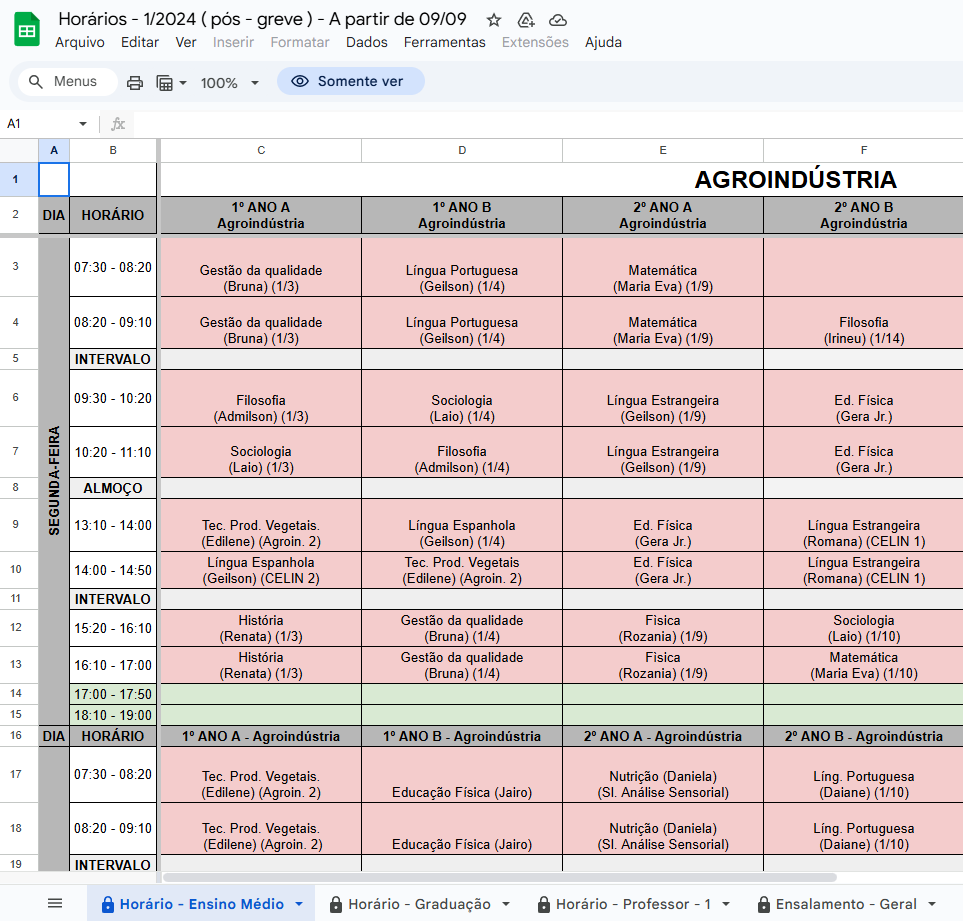
\includegraphics[width=0.9\textwidth]{figuras/plan-ant-1.png}
        \footnotesize Fonte: Elaborado pelo autor (2024)
    \end{minipage}
    \hfill
    \begin{minipage}{0.48\textwidth}
        \centering
        \captionof{figure}{Guia ``Horário - Graduação''}
        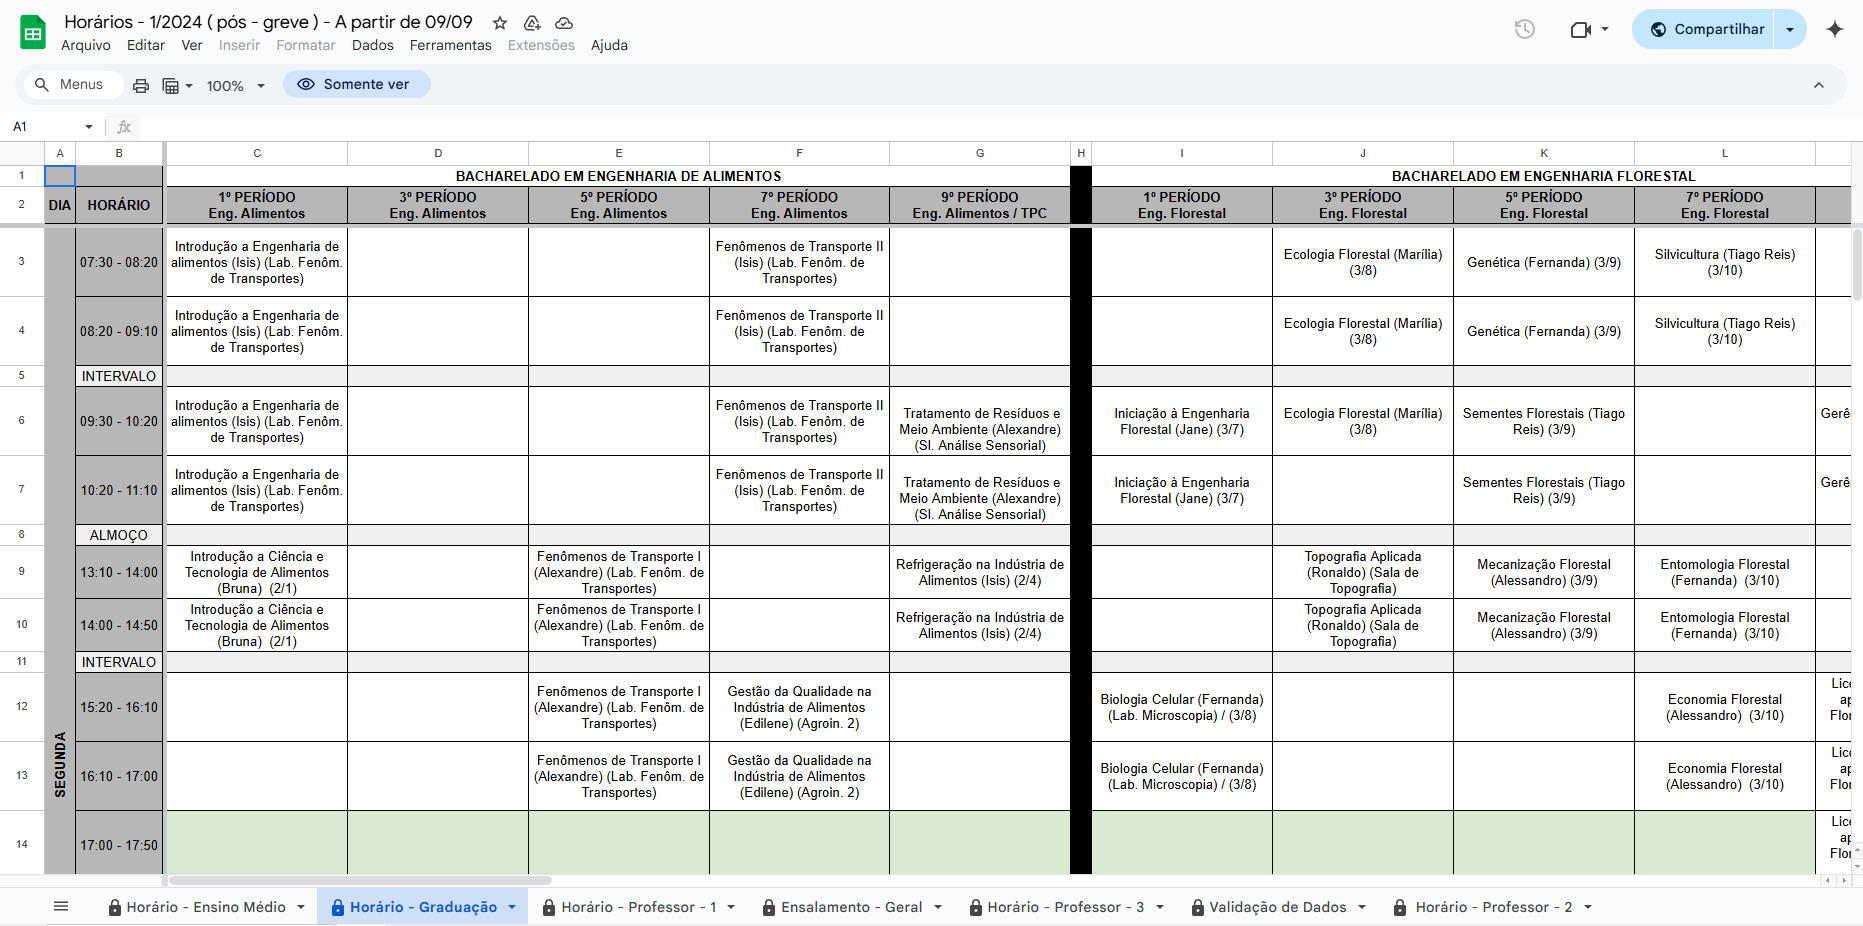
\includegraphics[width=0.9\textwidth]{figuras/plan-ant-2.png}
        \footnotesize Fonte: Elaborado pelo autor (2024)
    \end{minipage}
\end{frame}

\begin{frame}{Levantamento de Requisitos}
    \begin{itemize}
        \item Documentação: \vspace{0.5cm}
              \begin{enumerate}
                  \setcounter{enumi}{2}
                  \item Solução proposta; \vspace{0.5cm}
                  \item Funcionalidades desejadas. \vspace{0.5cm}
              \end{enumerate}
    \end{itemize}
\end{frame}

\begin{frame}{Front-end}
    \begin{itemize}
        \item Protótipo: \vspace{0.5cm}
              \begin{itemize}
                  \item Figma; \vspace{0.5cm}
              \end{itemize}
        \item Desenvolvimento: \vspace{0.5cm}
              \begin{itemize}
                  \item Next.js; \vspace{0.5cm}
                  \item Tailwind CSS. \vspace{0.5cm}
              \end{itemize}
        \item Justificativa. \vspace{0.5cm}
    \end{itemize}
\end{frame}

\begin{frame}{Back-end}
    \begin{itemize}
        \item Google Sheets como banco de dados: \vspace{0.5cm}
              \begin{itemize}
                  \item Benefícios; \vspace{0.5cm}
                  \item Processo de Atualização dos Dados: \vspace{0.5cm}
                        \begin{itemize}
                            \item O setor de ensino copia os dados mais recentes de uma planilha privada; \vspace{0.5cm}
                            \item Os dados são colados na planilha utilizada como banco de dados. \vspace{0.5cm}
                        \end{itemize}
              \end{itemize}
    \end{itemize}
\end{frame}

\begin{frame}{Back-end}
    \begin{itemize}
        \item Implementação: \vspace{0.5cm}
              \begin{itemize}
                  \item Spring Boot: \vspace{0.5cm}
                        \begin{itemize}
                            \item Essencial para estabelecer a conexão com a API do Google Sheets; \vspace{0.5cm}
                            \item Para garantir a segurança, configurada para permitir apenas operações de leitura. \vspace{0.5cm}
                        \end{itemize}
              \end{itemize}
        \item Arquitetura; \vspace{0.5cm}
        \item Justificativa. \vspace{0.5cm}
    \end{itemize}
\end{frame}

\begin{frame}{Integração Front-end com Back-end}
    \begin{itemize}
        \item Por meio de uma API RESTful; \vspace{0.5cm}
        \item Envio e retorno de dados; \vspace{0.5cm}
        \item Alterações feitas no Google Sheets apareceram automaticamente na plataforma; \vspace{0.5cm}
        \item Segurança e controle de acesso. \vspace{0.5cm}
    \end{itemize}
\end{frame}

\begin{frame}{Deploy}
    \begin{itemize}
        \item Front-end: Vercel; \vspace{0.5cm}
        \begin{itemize}
            \item Plataforma especializada no deploy de aplicações web baseadas em JavaScript. \vspace{0.5cm}
        \end{itemize}
        \item Back-end: Koyeb; \vspace{0.5cm}
        \begin{itemize}
            \item Plataforma serverless amigável para desenvolvedores. \vspace{0.5cm}
        \end{itemize}
    \end{itemize}
\end{frame}

\begin{frame}{Armazenamento do Código e Integração}
    \begin{itemize}
        \item Github; \vspace{0.5cm}
        \begin{itemize}
            \item Repositório de hospedagem de serviços Git. \vspace{0.5cm}
        \end{itemize}
        \item Conta vinculada com plataformas de deploy: \vspace{0.5cm}
              \begin{itemize}
                  \item Uso do Docker; \vspace{0.5cm}
              \end{itemize}
    \end{itemize}
\end{frame}

\begin{frame}{Ambiente de Desenvolvimento}
    \begin{itemize}
        \item Visual Studio Code; \vspace{0.5cm}
        \begin{itemize}
            \item Editor de código-fonte para auxiliar programadores na criação de softwares. \vspace{0.5cm}
        \end{itemize}
        \item Justificativa. \vspace{0.5cm}
    \end{itemize}
\end{frame}

\begin{frame}{Avaliação da Plataforma}
    \begin{itemize}
        \item Para avaliar a eficácia da plataforma; \vspace{0.5cm}
        \item Participação: Coordenador de Ensino Superior. \vspace{0.5cm}
    \end{itemize}
\end{frame}

\begin{frame}{Avaliação da Plataforma}
    \begin{itemize}
        \item A condução da entrevista foi realizada conforme os seguintes passos: \vspace{0.5cm}
              \begin{itemize}
                  \item Preparação: \vspace{0.5cm}
                        \begin{itemize}
                            \item Agendamento; \vspace{0.25cm}
                            \item Objetivos. \vspace{0.5cm}
                        \end{itemize}
                  \item Entrevista; \vspace{0.5cm}
                  \item Perguntas; \vspace{0.25cm}
                  \begin{itemize}
                    \item Com base no instrumento do TCC: ``SIGALAB: Sistema de Informação Gerencial Acadêmico para Reservas de Laboratórios''.
                  \end{itemize}
              \end{itemize}
    \end{itemize}
\end{frame}

\begin{frame}{Avaliação da Plataforma}
    \begin{itemize}
        \item Documentação: \vspace{0.5cm}
              \begin{enumerate}
                  \item Usabilidade e navegação; \vspace{0.5cm}
                  \item Eficiência na exibição dos horários; \vspace{0.5cm}
                  \item Redução de dificuldades operacionais; \vspace{0.5cm}
                  \item Satisfação geral; \vspace{0.5cm}
                  \item Melhorias e atualizações; \vspace{0.5cm}
                  \item Garantia de disponibilidade. \vspace{0.5cm}
              \end{enumerate}
    \end{itemize}
\end{frame}

\begin{frame}{Implementação de Melhorias e Atualizações}
    \begin{itemize}
        \item O histórico das versões desenvolvidas até o momento: \vspace{0.5cm}
              \begin{itemize}
                  \item v.1.0.0; \vspace{0.5cm}
                  \item v.2.0.0. \vspace{0.25cm}
                  \begin{itemize}
                    \item Criação de uma nova planilha no Google Sheets com as credenciais de login para acessar a tela de validação de dados; \vspace{0.25cm}
                    \item Implementação de uma nova tela para a validação dos dados da planilha dos horários; \vspace{0.25cm}
                    \item Adição de um botão no menu principal da plataforma para direcionar para validação de dados; \vspace{0.25cm}
                    \item Inclusão de três novos botões no menu principal da plataforma com links externos para os sistemas complementares. \vspace{0.25cm}
                  \end{itemize}
              \end{itemize}
    \end{itemize}
\end{frame}

\begin{frame}{Documentação}
    \begin{itemize}
        \item Para garantir a correta manutenção e funcionamento da plataforma; \vspace{0.5cm}
        \item Abordou os seguintes aspectos: \vspace{0.5cm}
              \begin{itemize}
                  \item Estrutura e organização dos dados; \vspace{0.5cm}
                  \item Regras para adição e atualização de informações; \vspace{0.5cm}
                  \item Padrões para nomes de guias e intervalos de células.
              \end{itemize}
    \end{itemize}
\end{frame}